% --------------------------------------------- %
% Q4) -- Aula 24 14/06
% --------------------------------------------- %
\subsection{Título da Subseção}
% Estrutura para escrever problemas
\begin{problem}
  Enunciado do Problema...
\end{problem}
\textcolor{deepGreen}{\textit{Solução:}}

Inserindo equação
\begin{align}
  \mathcal{M} &= -\frac{e^{2}\left(\bar{u}_{C} \gamma^{\mu}u_{A}\right)\left(\bar{u}_{D} \gamma_{\mu}u_{B}\right)}{\left(P_{A}-P_{C}\right)^{2}} + \frac{e^{2}\left(\bar{u}_{D} \gamma^{\mu}u_{A}\right)\left(\bar{u}_{C} \gamma_{\mu}u_{B}\right)}{\left(P_{A}-P_{D}\right)^{2}},
\end{align}
\newpage
Inserindo Figuras .TikZ
\begin{figure}[htb!]
  \centering
  \begin{tikzpicture}
    \begin{feynhand}
  \vertex[dot](v1) at (0,0){};
  \vertex[dot](v2) at (2,0){};

  \vertex[particle] (e_minus) [above left=of v1] {$\mathrm{e}^{-}$};
  \vertex[particle] (e_plus) [below left=of v1] {$\mathrm{e}^{+}$};
  \vertex[particle] (mu_plus) [above right=of v2] {$\mu^{+}$};
  \vertex[particle] (mu_minus) [below right=of v2] {$\mu^{-}$};

  \propag[antfer,mom={$k^{\prime}$}](e_plus) to (v1) {};
  \propag[fer,mom={$k$}](e_minus) to (v1) {};

  \propag[pho,mom={$q$}](v1) to (v2) {};

  \propag[fer,revmom={$p^{\prime}$}](mu_plus) to (v2) {};
  \propag[antfer,revmom={$p$}](mu_minus) to (v2) {};
\end{feynhand}

  \end{tikzpicture}
  \caption{Contribuição representativa do processo $e^{+}e^{-}\to \mu^{+} \mu^{-}$ em ordem dominante.}
  \label{fig:aniq-eletron-muon}
  % \legend{Fonte: O Autor}
\end{figure}

Inserindo Figuras .PNG
\begin{figure}[htb!]
  \begin{center}
    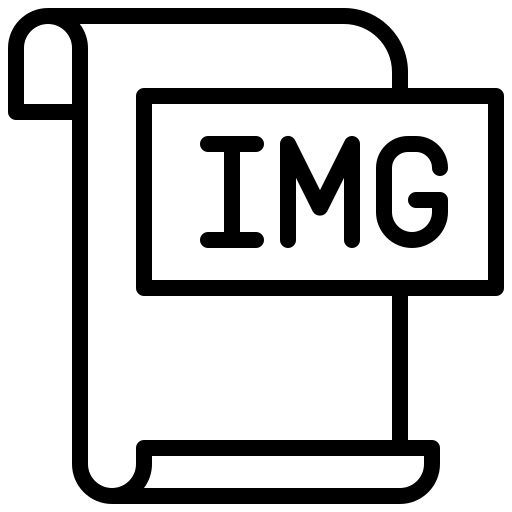
\includegraphics[width=0.5\textwidth]{img}
  \end{center}
  \caption{Imagem aleatória em .PNG}\label{fig:img}
\end{figure}


% --------------------------------------------- %
